\subsubsection{Heurística constructiva de cluster-first, route-second, clusterizando con algoritmo de K-means}

\subsubsubsection{Medición en base a tamaño del grafo}

En este caso, la heurística plantea que en peor caso tendremos k clusters igual a n, con una complejidad temporal de $\mathcal{O}(n^{2} * log(n))$. Es por ello que en algunos casos podemos tener k clusters menores a n, por ello, es de esperar un gráfico con variaciones.

\begin{figure}[H]
	\centering
	\begin{minipage}[t]{.45\textwidth}
		\centering
		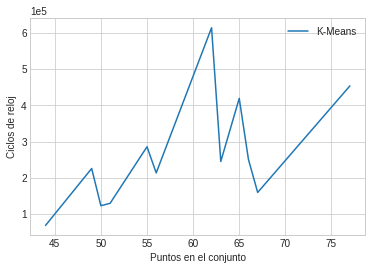
\includegraphics[scale=0.55]{exercise5/kmeans3}
	\end{minipage}\qquad
	\begin{minipage}[t]{.45\textwidth}
		\centering
		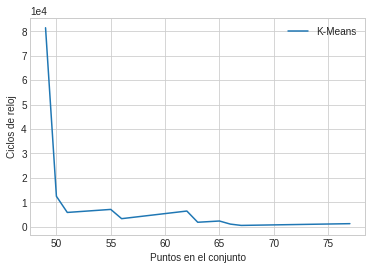
\includegraphics[scale=0.55]{exercise5/kmeansAcotado}
	\end{minipage}
\end{figure}

Tal como era de esperar, el gráfico no presenta una curva de crecimiento continuo a medida que crece el valor de n. Sin embargo, en el gráfico de la derecha vemos como la curva que representa a los puntos del gráfico del lado izquierdo, divididos por la cota de complejidad temporal, converge. Esto muestra que la heurística respeta la complejidad temproal planteada.

Luego, podemos concluir que la distribución de los puntos afecta en gran parte a la performance del algoritmo.


\subsubsubsection{Medición en base a distribución del grafo}

\begin{figure}[H]
	\centering
	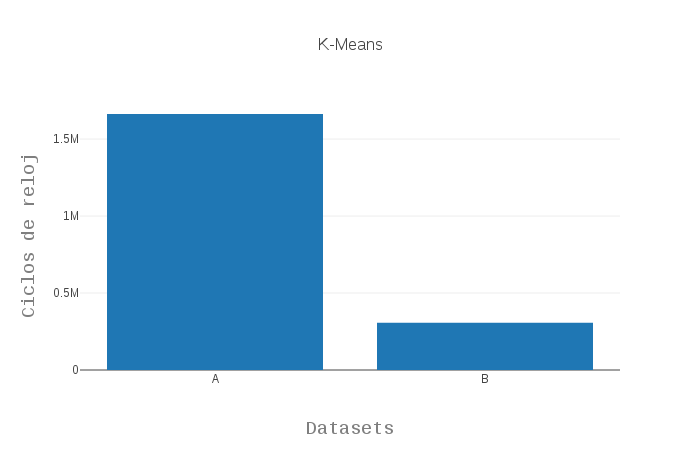
\includegraphics[scale=0.4]{exercise5/kmeansType.png}
\end{figure}